
        
\subsection{Decreasing rules}
\label{nwf:sec:decreasing_rules}
The definition below adapts the concept of decreasing rules from~\cite{endrullis2024generalized_arxiv_v2}. The difference lies in the treatment of weight comparisons for uniformly decreasing and closure decreasing rules: instead of directly comparing weights, we evaluate the difference between weights relative to the homomorphism $\mu$ of the strongly monotonic measurable semirings.
%  This difference must exceed a fixed positive constant $\delta \in \mathbb{R}_{>0}$.

\begin{definition}[Decreasing Rules]
    \label{nwf:def:decreasing_rule}
    Let $\mathcal{T} = (T,\mathbb{E}, (S, \oplus, \odot, 0_S, 1_S, \prec, \mu), w)$ be a finitary weighted type graph, \(\mathfrak{F}\) a DPO rewriting framework, $\rho = (L \overset{l}{\leftarrow} K \overset{r}{\rightarrow} R)$ a DPO rewriting rule, and $\delta \in \mathbb{R}_{>0}$. 

    \noindent
    The rule $\rho$ is \textbf{weakly decreasing} w.r.t. $\mathcal{T}$ in $\mathfrak{F}$ if 
            for every $t_K : K \to T$,
                $$ 
                  w_\mathcal{T}(\{l \star - = t_K\}) \succeq w_\mathcal{T}(\{r\star - = t_K\})$$
           
    \noindent
    The rule $\rho$ is \textbf{$\delta$-uniformly decreasing} w.r.t. $\mathcal{T}$ in $\mathfrak{F}$ if the following hold:
        \begin{itemize}
            \item[]- there exists a context closure $c_\rho$ for $\rho$ and $\mathcal{T}$ in $\mathfrak{F}$, 
            \item[]- for every $t_K : K \to T$,
            \begin{itemize}
                \item[] $\bullet$ $\{l \star - = t_K\} = \emptyset = \{r \star - = t_K\}$, or
                \item[] $\bullet$ $\mu(w_\mathcal{T}(\{l \star - = t_K\}))  >_{\mathbb{R}^+}   \mu(w_\mathcal{T}(\{r \star - = t_K\})) + \delta$.
            \end{itemize}
        \end{itemize}  
         
    \noindent
    The rule $\rho$ is
            \textbf{$\delta$-closure decreasing} w.r.t. $\mathcal{T}$ in $\mathfrak{F}$ if the following hold:
            \begin{itemize}
                \item[]- $S$ is strictly monotonic measurable semiring,
                \item[]- $\rho$ is weakly decreasing,
                \item[]- there exists a context closure $c_\rho$ for $\rho$ and $\mathcal{T}$ in $\mathfrak{F}$,
                \item[]- $ \mu(w_\mathcal{T}(\{l \star - = t_K\}))  >_{\mathbb{R}^+}  \mu(w_\mathcal{T}(\{r \star - = t_K\}))  + \delta$ for $t_K = l \star c_\rho$.
            \end{itemize}
\end{definition}

\begin{example}
    \label{nwf:example:decreasing_rule}
    Consider the DPO rule in~\autoref{ex:grsaa} shown below
     \begin{center} 
      \resizebox{0.7\textwidth}{!}{
      \begin{tikzpicture}
          \graphbox{$L$}{0mm}{0mm}{34mm}{15mm}{2mm}{-5mm}{
              \coordinate (o) at (0mm,-3mm); 
              \node[draw,circle] (l1) at ($(o)+(-10mm,0mm)$) {1};
              \node[draw,circle] (l2) at ($(l1)+(2,0)$) {2};
              \node[draw,circle] (l3) at ($(l1) + (1,0)$) {3};
              \draw[->] (l1) -- (l3) node[midway,above] {a};
              \draw[->] (l3) -- (l2) node[midway,above] {a};
          }     
          \graphbox{$K$}{40mm}{0mm}{24mm}{15mm}{2mm}{-5mm}{
              \coordinate (o) at (5mm,-3mm); 
              \node[draw,circle] (l1) at ($(o)+(-10mm,0mm)$) {1};
              \node[draw,circle] (l2) at ($(l1)+(1,0)$) {2};
              % \node[draw,circle] (l3) at ($(l1) + (1,0)$) {$\ $};
              % \draw[->] (l1) -- (l3) node[midway,above] {a};
              % \draw[->] (l3) -- (l2) node[midway,above] {a};
          }    
          \graphbox{$R$}{70mm}{0mm}{45mm}{15mm}{2mm}{-5mm}{
              \coordinate (o) at (-5mm,-3mm); 
              \node[draw,circle] (l1) at ($(o)+(-10mm,0mm)$) {1};
              \node[draw,circle] (l2) at ($(l1)+(3,0)$) {2};
              \node[draw,circle] (l3) at ($(l1) + (1,0)$) {4};
              \node[draw,circle] (l4) at ($(l1) + (2,0)$) {5};
              \draw[->] (l1) -- (l3) node[midway,above] {a};
              \draw[->] (l3) -- (l4) node[midway,above] {b};
              \draw[->] (l4) -- (l2) node[midway,above] {a};
          }    
          \node () at (37mm,-8mm) {$\overset{l}{\leftarrowtail}$};
          \node () at (67mm,-8mm) {$\overset{r}{\rightarrowtail}$};
          % \draw[>->] (51mm,2mm) -- (52mm,3mm);
      \end{tikzpicture}
      }
  \end{center}
   and the weighted type graph in \autoref{nwf:example:weighted_type_graph} over the real arithmetic semiring $\mathfrak{N}' = (\mathbb{R}^+,+,*,0_\mathbb{R},1_\mathbb{R},<,\operatorname{id}_{\mathbb{R}^+})$ shown below
    \begin{center}
        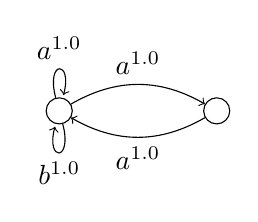
\begin{tikzpicture}
            \graphbox{}{0mm}{0mm}{32mm}{28mm}{-10mm}{-14mm}{
                \node[draw,circle] (1) at (0,0) {};
                \node[draw,circle] (2) at (2,0) {};
                \draw[->] (1) edge[loop above] node[midway, above] {$a^{1.0}$} (1) ;
                \draw[->] (1) edge[loop below] node[midway, below] {$b^{1.0}$} (1) ;
                \draw[->] (1) edge[bend left] node[midway, above] {$a^{1.0}$}  (2)  ;
                \draw[->] (2) edge[bend left] node[midway, below] {$a^{1.0}$} (1)   ;
            }
        \end{tikzpicture}
    \end{center}
     There are $t_K^{11}, t_K^{12}, t_K^{21}, t_K^{22}:K \rightarrow T$ as depicted below:

    \begin{center}
        \resizebox{0.49\textwidth}{!}{
            \begin{tikzpicture}
            \graphbox{\( K \)}{-50mm}{0mm}{40mm}{30mm}{2mm}{-6mm}{
                \coordinate (o) at (0mm,-10mm); 
                \node[draw,circle] (l1) at ($(o)+(-10mm,0mm)$) {1};
                \node[draw,circle] (l2) at ($(l1)+(2,0)$) {2};
                % \node[draw,circle] (l3) at ($(l1) + (1,0)$) {3};
                % \draw[] (l1) -- (l3) node[midway,above] {a};
                % \draw[] (l3) -- (l2) node[midway,above] {a};
            } 
                \graphbox{$T$}{0mm}{0mm}{40mm}{30mm}{-10mm}{-15mm}{
                    \node[draw,circle] (1) at (0,0) {$1\ 2$};
                    \node[draw,circle] (2) at (2,0) {};
                    \draw[->] (1) edge[loop above] node[midway, above] {$a$} (1) ;
                    \draw[->] (1) edge[loop below] node[midway, below] {$b$} (1) ;
                    \draw[->] (1) edge[bend left] node[midway, above] {$a$}  (2)  ;
                    \draw[->] (2) edge[bend left] node[midway, below] {$a$} (1)   ;
                }
                \node () at (-5mm,-15mm) {$\overset{t_K^{11}}{\to}$};
            \end{tikzpicture}
            } 
            \resizebox{0.49\textwidth}{!}{
            \begin{tikzpicture}
                \graphbox{\( K \)}{-50mm}{0mm}{40mm}{30mm}{2mm}{-6mm}{
                \coordinate (o) at (0mm,-10mm); 
                \node[draw,circle] (l1) at ($(o)+(-10mm,0mm)$) {1};
                \node[draw,circle] (l2) at ($(l1)+(2,0)$) {2};
                % \node[draw,circle] (l3) at ($(l1) + (1,0)$) {3};
                % \draw[] (l1) -- (l3) node[midway,above] {a};
                % \draw[] (l3) -- (l2) node[midway,above] {a};
            } 
                \graphbox{$T$}{0mm}{0mm}{40mm}{30mm}{-10mm}{-15mm}{
                    \node[draw,circle] (1) at (0,0) {$1$};
                    \node[draw,circle] (2) at (2,0) {2};
                    \draw[->] (1) edge[loop above] node[midway, above] {$a$} (1) ;
                    \draw[->] (1) edge[loop below] node[midway, below] {$b$} (1) ;
                    \draw[->] (1) edge[bend left] node[midway, above] {$a$}  (2)  ;
                    \draw[->] (2) edge[bend left] node[midway, below] {$a$} (1)   ;
                }
                \node () at (-5mm,-15mm) {$\overset{t_K^{12}}{\to}$};
            \end{tikzpicture}
            }
            \hspace{5mm}
            
            \resizebox{0.49\textwidth}{!}{
            \begin{tikzpicture}
                \graphbox{\( K \)}{-50mm}{0mm}{40mm}{30mm}{2mm}{-6mm}{
                \coordinate (o) at (0mm,-10mm); 
                \node[draw,circle] (l1) at ($(o)+(-10mm,0mm)$) {1};
                \node[draw,circle] (l2) at ($(l1)+(2,0)$) {2};
                % \node[draw,circle] (l3) at ($(l1) + (1,0)$) {3};
                % \draw[] (l1) -- (l3) node[midway,above] {a};
                % \draw[] (l3) -- (l2) node[midway,above] {a};
            } 
                \graphbox{$T$}{0mm}{0mm}{40mm}{30mm}{-10mm}{-15mm}{
                    \node[draw,circle] (1) at (0,0) {2};
                    \node[draw,circle] (2) at (2,0) {1};
                    \draw[->] (1) edge[loop above] node[midway, above] {$a$} (1) ;
                    \draw[->] (1) edge[loop below] node[midway, below] {$b$} (1) ;
                    \draw[->] (1) edge[bend left] node[midway, above] {$a$}  (2)  ;
                    \draw[->] (2) edge[bend left] node[midway, below] {$a$} (1)   ;
                }
                \node () at (-5mm,-15mm) {$\overset{t_K^{21}}{\to}$};
            \end{tikzpicture}
            }
            \resizebox{0.49\textwidth}{!}{
            \begin{tikzpicture}
                \graphbox{\( K \)}{-50mm}{0mm}{40mm}{30mm}{2mm}{-6mm}{
                \coordinate (o) at (0mm,-10mm); 
                \node[draw,circle] (l1) at ($(o)+(-10mm,0mm)$) {1};
                \node[draw,circle] (l2) at ($(l1)+(2,0)$) {2};
                % \node[draw,circle] (l3) at ($(l1) + (1,0)$) {3};
                % \draw[] (l1) -- (l3) node[midway,above] {a};
                % \draw[] (l3) -- (l2) node[midway,above] {a};
            } 
                \graphbox{$T$}{0mm}{0mm}{40mm}{30mm}{-10mm}{-15mm}{
                    \node[draw,circle] (1) at (0,0) {};
                    \node[draw,circle] (2) at (2,0) {$1\ 2$};
                    \draw[->] (1) edge[loop above] node[midway, above] {$a$} (1) ;
                    \draw[->] (1) edge[loop below] node[midway, below] {$b$} (1) ;
                    \draw[->] (1) edge[bend left] node[midway, above] {$a$}  (2)  ;
                    \draw[->] (2) edge[bend left] node[midway, below] {$a$} (1)   ;
                }
                \node () at (-5mm,-15mm) {$\overset{t_K^{22}}{\to}$};
            \end{tikzpicture}
            }
      \end{center}
    The set $\{l \star - = t_K^{11}\}$ has two morphisms $h_{11}^1$ and $h_{11}^2$ as illustrated below:
    \begin{center}
        \resizebox{0.49\textwidth}{!}{
        \begin{tikzpicture}
          \graphbox{\( L \)}{-50mm}{0mm}{40mm}{40mm}{2mm}{-6mm}{
            \coordinate (o) at (0mm,-10mm); 
            \node[draw,circle] (l1) at ($(o)+(-10mm,0mm)$) {1};
            \node[draw,circle] (l2) at ($(l1)+(2,0)$) {2};
            \node[draw,circle] (l3) at ($(l1) + (1,0)$) {3};
            \draw[] (l1) -- (l3) node[midway,above] {a};
            \draw[] (l3) -- (l2) node[midway,above] {a};
        } 
            \graphbox{$T$}{0mm}{0mm}{40mm}{40mm}{-10mm}{-17mm}{
                \node[draw,circle] (1) at (0,0) {$1\ 2$};
                \node[draw,circle] (2) at (2,0) {3};
                \draw[->] (1) edge[loop above] node[midway, above] {$a^{1.0}$} (1) ;
                \draw[->] (1) edge[loop below] node[midway, below] {$b^{1.0}$} (1) ;
                \draw[->] (1) edge[bend left] node[midway, above] {$a^{1.0}$}  (2)  ;
                \draw[->] (2) edge[bend left] node[midway, below] {$a^{1.0}$} (1)   ;
            }
            \node () at (-5mm,-15mm) {$\overset{h_{11}^1}{\to}$};
        \end{tikzpicture}
        }
        \resizebox{0.49\textwidth}{!}{
            \begin{tikzpicture}
              \graphbox{\(L\)}{-50mm}{0mm}{40mm}{40mm}{2mm}{-10mm}{
                \coordinate (o) at (0mm,-10mm); 
                \node[draw,circle] (l1) at ($(o)+(-10mm,0mm)$) {1};
                \node[draw,circle] (l2) at ($(l1)+(2,0)$) {2};
                \node[draw,circle] (l3) at ($(l1) + (1,0)$) {3};
                \draw[] (l1) -- (l3) node[midway,above] {a};
                \draw[] (l3) -- (l2) node[midway,above] {a};
            } 
                \graphbox{$T$}{0mm}{0mm}{40mm}{40mm}{-10mm}{-20mm}{
                    \node[draw,circle] (1) at (0,0) {$1\ 2\ 3$};
                    \node[draw,circle] (2) at (2,0) {};
                    \draw[->] (1) edge[loop above] node[midway, above] {$a^{1.0}$} (1) ;
                    \draw[->] (1) edge[loop below] node[midway, below] {$b^{1.0}$} (1) ;
                    \draw[->] (1) edge[bend left] node[midway, above] {$a^{1.0}$}  (2)  ;
                    \draw[->] (2) edge[bend left] node[midway, below] {$a^{1.0}$} (1)   ;(1)   ;
                }
                \node () at (-5mm,-15mm) {$\overset{h_{11}^2}{\to}$};
            \end{tikzpicture}
            }
      \end{center}
    Therefore, we have \begin{flalign*}
        w_\mathcal{T}(\{l \star - = t_K^{11}\})
        =&w_\mathcal{T}(\{h_{11}^1, h_{11}^2\})\\
        \overset{\mathrm{def}}{=}&w_\mathcal{T}(h_{11}^1) + w_\mathcal{T}(h_{11}^2) \\
        =&(1.0^1 * 1.0^1) + (1.0^1 * 1.0^1)\\
        =&2.0
    \end{flalign*}
    The set $\{r \star - = t_K^{11}\}$ has one morphism $h_{11}^3$ as illustrated below:
    \begin{center}
        \resizebox{0.49\textwidth}{!}{
        \begin{tikzpicture}
          \graphbox{\( R \)}{-55mm}{0mm}{45mm}{44mm}{1mm}{-22mm}{
            \coordinate (o) at (-5mm,-3mm); 
            \node[draw,circle] (l1) at ($(o)+(-10mm,0mm)$) {1};
            \node[draw,circle] (l2) at ($(l1)+(3,0)$) {2};
            \node[draw,circle] (l3) at ($(l1) + (1,0)$) {4};
            \node[draw,circle] (l4) at ($(l1) + (2,0)$) {5};
            \draw[->] (l1) -- (l3) node[midway,above] {a};
            \draw[->] (l3) -- (l4) node[midway,above] {b};
            \draw[->] (l4) -- (l2) node[midway,above] {a};
        } 
            \graphbox{$T$}{0mm}{0mm}{40mm}{44mm}{-10mm}{-22mm}{
                \node[draw,circle] (1) at (0,0) {$1\ 2\ 4\ 5$};
                \node[draw,circle] (2) at (2,0) {};
                \draw[->] (1) edge[loop above] node[midway, above] {$a^{1.0}$} (1) ;
                \draw[->] (1) edge[loop below] node[midway, below] {$b^{1.0}$} (1) ;
                \draw[->] (1) edge[bend left] node[midway, above] {$a^{1.0}$}  (2)  ;
                \draw[->] (2) edge[bend left] node[midway, below] {$a^{1.0}$} (1)   ;
            }
            \node () at (-5mm,-19mm) {$\overset{h_{11}^3}{\to}$};
        \end{tikzpicture}
        }
      \end{center}
    Therefore, we have: $w_\mathcal{T}(\{r \star - = t_K^{11}\}) = w_\mathcal{T}(h_{11}^3) = 1.0^1 * 1.0^1 * 1.0 ^ 1 = 1.0$. Thus, we have $w_\mathcal{T}(\{l \star - = t_K^{11}\}) = 2.0 \geq 1.0 = w_\mathcal{T}(\{r \star - = t_K^{11}\})$.

    Similarly, we can check that $w_\mathcal{T}(\{l \star - = t_K^{12}\}) = 1.0 \geq 1.0 = w_\mathcal{T}(\{r \star - = t_K^{12}\})$,  $w_\mathcal{T}(\{l \star - = t_K^{21}\}) = 1.0 \geq 1.0 = w_\mathcal{T}(\{r \star - = t_K^{21}\})$, and $w_\mathcal{T}(\{l \star - = t_K^{22}\}) = 1.0 \geq 1.0 = w_\mathcal{T}(\{r \star - = t_K^{22}\})$. The rule is therefore weakly decreasing.

    There exists a context closure $c$ for the DPO rule in the weighted type graph, by \autoref{wf:example:context_closure}, shown below 
    \begin{center}
    \resizebox{0.6\textwidth}{!}{
    \begin{tikzpicture}
      \graphbox{\( L \)}{-50mm}{0mm}{40mm}{40mm}{2mm}{-8mm}{
        \coordinate (o) at (0mm,-10mm); 
        \node[draw,circle] (l1) at ($(o)+(-10mm,0mm)$) {1};
        \node[draw,circle] (l2) at ($(l1)+(2,0)$) {2};
        \node[draw,circle] (l3) at ($(l1) + (1,0)$) {3};
        \draw[] (l1) -- (l3) node[midway,above] {a};
        \draw[] (l3) -- (l2) node[midway,above] {a};
    } 
        \graphbox{$T$}{0mm}{0mm}{40mm}{40mm}{-10mm}{-17mm}{
            % \node[draw,circle] (1) at (0,0) {$1\ 2\ 3$};
            % \node[draw,circle] (2) at (2,0) {};
            \coordinate (o) at (2mm,-3mm); 
            \node[draw,circle] (1) at ($(o)+(0,0mm)$) {$1\ 2\ 3$};
            \node[draw,circle] (2) at ($(o)+(2,0)$) {};
            \draw[->] (1) edge[loop above] node[midway, above] {$a^{1}$} (1) ;
            \draw[->] (1) edge[loop below] node[midway, below] {$b^{1}$} (1) ;
            \draw[->] (1) edge[bend left] node[midway, above] {$a^{1}$}  (2)  ;
            \draw[->] (2) edge[bend left] node[midway, below] {$a^{1}$} (1)   ;
        }
        \node () at (-5mm,-15mm) {$\overset{c}{\to}$};
    \end{tikzpicture}
    }
  \end{center}
    Since we have additionally $t_K^{11} = l \star c$ and $w_\mathcal{T}(\{l \star - = t_K^{11}\}) = 2.0 > 1.0 + \delta = w_\mathcal{T}(\{r \star - = t_K^{11}\}) + \delta$ for $0 < \delta < 1.0$, the rule is $\delta$-closure decreasing with $0 < \delta < 1.0$ since the semiring is strictly monotonic measurable.
\end{example} 

The following lemma guaranteeing that, under certain constraints: exact weights of host graphs can be computed, and upper bounds for result-graph weights can be derived. 
\begin{lemma}[\cite{endrullis2024generalized_arxiv_v2}]
    \label{nwf:lem_4d13}
\ \newline
\begin{minipage}{0.7\textwidth}
    Let $\mathcal{T} = (T,\mathbb{E}, (S, \oplus, \odot, 0_S, 1_S, \prec, \mu), w)$ be a finitary weighted type graph. Consider the pushout square $\delta$ illustrated on the right. We define
\end{minipage}
\begin{minipage}{0.3\textwidth}
    \begin{center}{\normalfont
        \begin{tikzpicture}[node distance=12mm]
            \node (A) {$A$};
            \node (B) [right of=A] {$B$};
            \node (C) [below of=A] {$C$};
            \node (D) [right of=C] {$D$};
            
            \draw [->] (A) to node [above, label] {$\alpha$} (B);
            \draw [->] (A) to node [left, label] {$\beta$} (C);
            \draw [->] (B) to node [right, label] {$\beta'$} (D);
            \draw [->] (C) to node [below, label] {$\alpha'$} (D);
            
            \node [at=($(A)!.5!(D)$)] {$\delta$};
        \end{tikzpicture}
    }\end{center}
\end{minipage}
     \[k = \underset{t_A:A \rightarrow T}{\bigoplus}
            \left ( 
                \underset{\substack{t_C:C \rightarrow T\\
                                            t_A = \beta \star t_C }}{\bigoplus}
                        w_\mathcal{T}(t_C - \beta)     
                 \right ) 
            \odot 
                w_\mathcal{T}(\set{\alpha \star - = t_A})
    \]
    The following conditions hold
    \begin{enumerate}[label=(\Alph*)]
        \item  $w_\mathcal{T}(D)=k$ if $\delta$ is weighable with $\mathcal{T}$.
        \item  $w_\mathcal{T}(D)\preceq k$ if $\delta$ is bounded above by $\mathcal{T}$  and \(w(e) \succeq 1_S\) for all $e \in \mathbb{E}$.
    \end{enumerate}
\end{lemma}

Adapted from \cite[Theorem C.3]{endrullis2024generalized_arxiv_v2}, the lemma below relates decreasing rules to weight reduction under specific constraints. 
\begin{lemma}[Decreasing steps]
    \label{nwf:lem:decreasing_step}
\ \newline
\begin{minipage}{0.7\textwidth}
    Let $\mathcal{T} = (T,\mathbb{E}, (S, \oplus, \odot, 0_S, 1_S, \prec, \mu), w)$ be a finitary weighted type graph, $\rho$ a rewriting rule and $\Delta \in \mathfrak{F}(\rho)$ a DPO diagram
    (shown on the right)   such that the following conditions hold:
\end{minipage}  
\begin{minipage}{0.3\textwidth}
    \begin{center}
        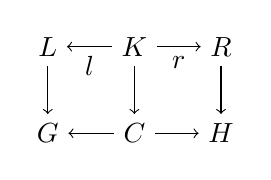
\begin{tikzpicture}[node distance=11mm]
          \node (I) {$K$};
          \node (L) [left of= I] {$L$};
          \node (R) [right of=I] {$R$}; 
          \node (G) [below of=L] {$G$};
          \node (C) [below of=I] {$C$};
          \node (H) [below of=R] {$H$};
        %   \node (T) [left=of $(L)!0.5!(G)$] {$T$};
        %   \draw [->] (L) to  node [label, above] {$c$}  (T);
        %   \draw [->] (G) to  node [label, below] {$\alpha$} (T);
          \draw [->] (I) to node [label, below] {$l$} (L);
          \draw [->] (I) to node [label, below] {$r$} (R);
          \draw [->] (L) to  (G);
          \draw [->] (I) to (C);
          \draw [->] (R) to (H);
          \draw [->] (C) to (G);
          \draw [->] (C) to (H);
        \end{tikzpicture}
      \end{center}
\end{minipage}
   \begin{itemize}
       \item $\operatorname{left}(\Delta)$ is weighable with \(\mathcal{T}\), and
       \item $\operatorname{right}(\Delta)$ is bounded above by \(\mathcal{T}\), and
       \item $w(e) \succeq 1_S$ for all $e \in \mathbb{E}$.
   \end{itemize}

   \noindent
  We have:
   \begin{itemize}
       \item $\mu(w_\mathcal{T}(G)) \succeq \mu(w_\mathcal{T}(H))$ if $\rho$ is weakly decreasing,
       \item $\mu(w_\mathcal{T}(G)) >_{\mathbb{R}^+} \mu(w_\mathcal{T}(H)) + \delta$ if $\rho$ is $\delta$-uniformly or $\delta$-closure decreasing for some $\delta >_{\mathbb{R}^+} 0$ and $w(e) \succeq 1_S$ for all $e \in \mathbb{E}$.
   \end{itemize}
\end{lemma} 

\begin{proof}
    \label{nwf:proof:decreasing_step}
    \noindent For every \( t_K: K \rightarrow T \), we define
$
        S_{t_K} \overset{\operatorname{def}}{=}   
        \underset{\substack{t_C:C \rightarrow T \\
        t_K = h_{KC} \star t_C }}{\bigoplus} 
        w_\mathcal{T}(t_C - h_{KC})  
$.
    
    \noindent For all $t_K: K \to T$ and $X,Y \in S$, the following claims hold:
    \begin{enumerate}[label=(\alph*)] 
        \item \label{s_nz} $S_{t_K} \ne 0_S$ if there is $t_C$ with $ t_K = h_{KC} \star t_C$.  
        \begin{proof}
            By definition of weighted type graph, for all $e \in \mathbb{E}$, we have 
            \begin{flalign}
                w(e) \neq 0_S \label{eq_we_neq_0s1111}
            \end{flalign}
            For every $t_C:C \to T$, we have 
            \begin{flalign*}
                &w_\mathcal{T}(t_C - h_{KC}) \\
               =&\bigodot_{e\in \mathbb{E}} w_e(t_C - h_{KC}) 
                 \hspace{2cm}\text{by \autoref{def:weight_excluding}}\\
               =&\bigodot_{e\in \mathbb{E}} 
                 \bigodot_{\substack{\alpha \in \{- * t_C = e\}\\
                    \alpha \notin \left\{ \iota \in \operatorname{Hom}(X, C)~\middle|~\exists \zeta:X \to K,~\zeta \star h_{KC} = \iota \right\}
                 }
                 } w(e)  \hspace{2cm} \text{by~\autoref{def:weight_excluding_pre}} 
                 \\
               \neq&0_S \hspace{0.5cm}\text{by Equation~\eqref{eq_we_neq_0s1111},~\autoref{prop_endrullis_2d7}\eqref{eq:prop_neq0_mul_neq0} and~\autoref{def:bigodot}}  
            \end{flalign*}

            Therefore, $S_{t_K} \overset{\operatorname{def}}{=}   
            \underset{\substack{t_C:C \rightarrow T \\
            t_K = h_{KC} \star t_C }}{\bigoplus} 
            w_\mathcal{T}(t_C - h_{KC}) \neq 0_S$ if there exists be a morphism such that $t_K = h_{KC} \star t_C$ by~\autoref{prop_endrullis_2d7}\eqref{eq:prop_neq0_plus_neq0}.
            % For every $t_C:C \to T$ such that $t_K = h_{KC} \star t_C$, we have $w_\mathcal{T}(t_C - h_{KC}) \neq 0_S$ by \eqref{eq:prop_neq0_mul_neq0}. 
        \end{proof}
        
        \item \label{s_ge1} $S_{t_K} \succeq 1_S$ if there is $t_C$ with $ t_K = h_{KC} \star t_C$ and $w_\mathcal{T}(e) \succeq 1_S$ for all $e \in \mathbb{E}$,
        \begin{proof}
            By the definition of weighted type graph, for all $e \in \mathbb{E}$, we have $w(e) \neq 0_S$.  
            By assumption, we have $w_\mathcal{T}(e) \succeq 1_S$ for all $e \in \mathbb{E}$. Thus, we have 
            \begin{flalign}
                1_S \preceq w(e) \neq 0_S \label{eq_we_neq_0s_geq1_0}
            \end{flalign}
            By~\autoref{prop_endrullis_2d7}\eqref{eq:prop_neg0_ge1_mul_ge1}, we have
            \begin{flalign}
                1_S \preceq w_\mathcal{T}(t_C - h_{KC}) \label{eq_we_neq_0s_geq1}
            \end{flalign}

            Therefore, $S_{t_K} \overset{\operatorname{def}}{=}   
            \underset{\substack{t_C:C \rightarrow T \\
            t_K = h_{KC} \star t_C }}{\bigoplus} 
            w_\mathcal{T}(t_C - h_{KC}) \succeq 1_S$ if there exists be a morphism such that $t_K = h_{KC} \star t_C$ by~\autoref{def:real_strongly_monotonic_semiring}\eqref{ax:s1}.
        \end{proof}
        
        % \item \label{claim:le} $Y \succeq X \implies  Y \odot S_{t_K} \succeq X \odot S_{t_K}$
        % \\ by Axiom \eqref{ax:s3}. \todo{to delete: inutile}
         
        \item \label{claim:st} if there exists $t_C$ with $t_K = h_{KC} \star t_C$ then
        $$ \mu(Y) >_{\mathbb{R}^+} \mu(X) + \delta  \implies \mu(Y \odot S_{t_K}) >_{\mathbb{R}^+} \mu(X \odot S_{t_K})$$
                % $$\left (\exists \alpha \geq \delta.~\mu(Y) > \mu(X) + \alpha \right ) \implies (\mu(Y \odot S_{t_K}) > \mu(X \odot S_{t_K}))$$
        \begin{proof}
           Suppose that there is $t_C$ with $t_K = h_{KC} \star t_C$. We have $S_{t_K} \neq 0_S$ by Claim~\ref{s_nz}, and we conclude by~\autoref{def:real_strongly_monotonic_semiring}\eqref{ax:s4''}.
        \end{proof}
    
        \item \label{claim:sh_{DT}elta} 
        if there exists $t_C$ with $t_K = h_{KC} \star t_C$, and  $w_\mathcal{T}(e) \succeq 1_S$ for all $e \in \mathbb{E}$ then
        % $$\left (\exists \alpha \geq \delta.~\mu(Y) > \mu(X) +  \alpha \right ) \implies (\exists \beta \geq \delta. \mu(Y \odot S_{t_K}) > \mu(X \odot S_{t_K})  + \beta)$$
        $$\mu(Y) >_{\mathbb{R}^+} \mu(X) +  \delta \implies \mu(Y \odot S_{t_K}) >_{\mathbb{R}^+} \mu(X \odot S_{t_K})  + \delta $$
        \begin{proof}
            Suppose that there is $t_C$ with $t_K = h_{KC} \star t_C$. We have $1_S \preceq S_{t_K} \neq 0_S$ by Claim~\ref{s_nz} and Claim~\ref{s_ge1}, and we conclude by~\autoref{def:real_strongly_monotonic_semiring}\eqref{ax:s4'}. 
        \end{proof}

        \item \label{claim:0} 
        if there is no $t_C$ with $t_K = h_{KC} \star t_C$ then  $S_{t_K} = 0_S$, thus
        $$Y \odot S_{t_K} = 0_S = X \odot S_{t_K} $$
    
        \item \label{claim:exist_st} 
        If there is a context closure $t_L$ for $\rho$ and $T$ in $\mathfrak{F}$ , then, let $t_K = l \star t_L$, we have
        $$ \mu(Y) >_{\mathbb{R}^+} \mu(X) + \delta \implies \mu(Y \odot S_{t_K}) >_{\mathbb{R}^+} \mu(X \odot S_{t_K})$$
        \begin{proof}
            
       By \autoref{def:context_closure} of context closure, there exists $t_G : G \rightarrow T$ such that 
        \begin{flalign*}
             t_L = h_{LG} \star t_G \tag{1} \label{eq_tl_hlg_tg}
        \end{flalign*}
      i.e. we have the following commutative diagram
     
    \begin{center}
        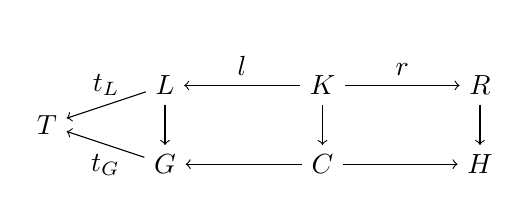
\begin{tikzpicture}[node distance=11mm]
          \node (I) at (0,0) {$K$};
          \node (L) at (-2,0) {$L$};
          \node (R) at (2,0) {$R$};
          \node (G) at (-2,-1) {$G$};
          \node (C) at (0,-1) {$C$};
          \node (H) at (2,-1) {$H$};
          \node (T) at (-3.5,-0.5) {$T$};
          \draw [->] (L) to  node [label, above] {$t_L$}  (T);
          \draw [->] (G) to  node [label, below] {$t_G$} (T);
          \draw [->] (I) to node [label, above] {$l$} (L);
          \draw [->] (I) to node [label,above] {$r$} (R);
        %   \draw [->] (L) to node [label, right] {$m$} (G);
        \draw [->] (L) to node [label, right] {} (G);
          \draw [->] (I) to (C);
          \draw [->] (R) to (H);
          \draw [->] (C) to (G);
          \draw [->] (C) to (H);
        \end{tikzpicture}
      \end{center}
    
        Let $t_C \overset{\operatorname{def}}{=} h_{CG} \star t_G$ and $t_K \overset{\operatorname{def}}{=} l \star t_L$. We have\\
        \begin{flalign*}
              t_K  &=  l \star t_L &\text{by definition of $t_K$}
            \\ &=   l \star (h_{LG}  \star t_G) & \text{by Equation~\eqref{eq_tl_hlg_tg}}
            \\ &= (l \star h_{LG}) \star t_G &\text{by associativity }
            \\ &= (h_{KC} \star h_{CG}) \star t_G & \text{by commutative of $\square KLGC$}
            \\ &= h_{KC} \star (h_{CG}  \star t_G) & \text{by associativity}
            \\ & = h_{KC} \star t_C &\text{by definition of $t_C$}
        \end{flalign*}
        and the claim follows from Claim~\ref{claim:st}, sinc $t_C$ is a morphism such that $t_K = h_{KC} \star t_C$.
    \end{proof}

        \item \label{claim:exist_sh_{DT}elta} 
        If there is a context closure $t_L$ for $\rho$ and $T$ in $\mathfrak{F}$, and $w_\mathcal{T}(e) \succeq 1_S$ for all $e \in \mathbb{E}$ then, let $t_K = l \star t_L$, we have 
            % $$\left (\exists \alpha \geq \delta. Y \succ X +  \alpha \right ) \implies (\exists \beta \geq \delta. Y \odot S_{t_K} \succ X \odot S_{t_K}  + \beta)$$
        $$\mu(Y) >_{\mathbb{R}^+} \mu(X) + \delta \implies \mu(Y \odot  S_{t_K}) \succ_{\mathbb{R}^+} \mu(X \odot  S_{t_K})  + \delta$$ 
        \begin{proof}
            The proof is analogous to the proof of Claim~\ref{claim:exist_st} but with Claim~\ref{claim:sh_{DT}elta} instead of Claim~\ref{claim:st} in the end.
        \end{proof} 
    \end{enumerate}
    
    \noindent For every \( t_K: K \rightarrow T \), let
    \begin{flalign*}
        \Lambda_{t_K} &\overset{\operatorname{def}}{=}  w_\mathcal{T}(\{l \star - = t_K\})
        \\
        \Omega_{t_K} &\overset{\operatorname{def}}{=}  w_\mathcal{T}(\{r \star - = t_K\})
    \end{flalign*}
  By \autoref{nwf:lem_4d13}, we have 
        \begin{flalign*} 
            w_\mathcal{T}(G) &=
                \underset{\substack{t_K: K \rightarrow T}}{\bigoplus}     \ \
            (S_{t_K} \odot \Lambda_{t_K})
              \\
            w_\mathcal{T}(H) &\preceq
            \underset{\substack{t_K: K \rightarrow T}}{\bigoplus}     \ \
                (S_{t_K} \odot \Omega_{t_K})
        \end{flalign*}

    \noindent We complete the proof with a analysis by cases:
    \begin{enumerate}
        \item  If $\rho$ is weakly decreasing, then, by \autoref{nwf:def:decreasing_rule} of weakly decreasing rule, we have $\Lambda_{t_K} \succeq \Omega_{t_K}$
        for every $t_K: K \rightarrow T$. 
        By~\autoref{def:real_strongly_monotonic_semiring}\eqref{ax:s3}, for every  $ t_K : K \rightarrow T$, we have 
                \begin{flalign*} 
                    S_{t_K} \odot \Lambda_{t_K} \succeq S_{t_K} \odot \Omega_{t_K} \tag{NE} \label{steps:weightC:ge} 
                \end{flalign*}
        Thus, we have $w_\mathcal{T}(G) \succeq w_\mathcal{T}(H)$, from~\autoref{def:real_strongly_monotonic_semiring}\eqref{ax:s1}.
        % \item
        %     If $\rho$ is $\delta$-uniformly decreasing for some $\delta \in \mathbb{R}_{>0}$, then, by \autoref{def:decreasing_rule} of $\delta$-uniformly decreasing rule,
        %     for all $t_K : K \to T$, we have 
        %                     \begin{itemize}                                
        %                         \item $\exists \alpha \geq \delta.~\mu(\Lambda_{t_K}) > \mu(\Omega_{t_K}) + \alpha$, or
        %                         \item $\{l \star - = t_K\} = \emptyset = \{r \star - = t_K\}$
        %                     \end{itemize}
        %     From \ref{claim:st} and \ref{claim:0}, for every \( t_K: K \rightarrow T \), we have
        %     \begin{enumerate}[label=(\roman*)]
        %         \item $S_{t_K} \odot \Lambda_{t_K} = 0_S =  S_{t_K} \odot \Omega_{t_K}$, or        
        %         \item  \label{it:strict} $ \mu(\Lambda_{t_K} \odot S_{t_K}) >  \mu(S_{t_K} \odot \Omega_{t_K})$
        %     \end{enumerate}
        %     To establish $ \mu(w_\mathcal{T}(G)) > \mu(w_\mathcal{T}(H))$, using \eqref{ax:s2}, 
        %     it suffices to show that we have case~\ref{it:strict} for some $t_K : K \to T$.
        %     This follows from \ref{claim:exist_st} since we have a context closure for $\rho$ and $\mathcal{T}$, by assumption.
        \item  
            Suppose that $\rho$ is $\delta$-uniformly decreasing for $\delta \in \mathbb{R}_{>0}$, and $w_\mathcal{T}(e) \succeq 1_S$ for all $e \in \mathbb{E}$. By \autoref{nwf:def:decreasing_rule} of $\delta$-uniformly decreasing rule,
            for all $t_K : K \to T$, we have  
                            \begin{itemize}                                
                                \item $\mu(\Lambda_{t_K}) >_{\mathbb{R}^+} \mu(\Omega_{t_K}) + \delta$,
                                % $\exists \alpha \geq \delta  .~\mu(\Lambda_{t_K}) > \mu(\Omega_{t_K}) + \alpha$, 
                                 or
                                \item $\{l \star - = t_K\} = \emptyset = \{r \star - = t_K\}$
                            \end{itemize}
            From Claim~\ref{claim:sh_{DT}elta} and Claim~\ref{claim:0}, for every \( t_K: K \rightarrow T \), we obtain
            \begin{enumerate}[label=(\roman*)]
                \item $S_{t_K} \odot \Lambda_{t_K} = 0_S =  S_{t_K} \odot \Omega_{t_K}$, or
                \item  \label{it:strich_{DT}elta}  $\mu(\Lambda_{t_K} \odot S_{t_K}) >_{\mathbb{R}^+} \mu(\Omega_{t_K} \odot S_{t_K}) + \delta$
                % $\exists \beta \geq \delta  .\  \mu(\Lambda_{t_K} \odot S_{t_K}) > \mu(\Omega_{t_K} \odot S_{t_K}) + \beta$
            \end{enumerate}
            To establish $ \mu(w_\mathcal{T}(G)) >_{\mathbb{R}^+} \mu(w_\mathcal{T}(H)) + \delta$, using~\autoref{def:real_strongly_monotonic_semiring}\eqref{ax:s2'}, 
            it suffices to show that we have Case~\ref{it:strich_{DT}elta} for some $t_K : K \to T$.
            This follows from Claim~\ref{claim:exist_sh_{DT}elta} since we have a context closure for $\rho$ and $\mathcal{T}$ by assumption.
            % \item
            % If $\rho$ is $\delta$-closure decreasing, 
            % then it is also weakly decreasing and we obtain \eqref{steps:weightC:ge} for every $t_K : K \to T$.
            % Since the semiring is strictly ordered museurable, it suffices to show that there exists some $t_K : K \to T$ such that
            % \begin{align}
            %    \mu( S_{t_K} \odot \Lambda_{t_K})  \succ \mu(S_{t_K} \odot \Omega_{t_K})
            %   \tag{$\star$} \label{steps:weightC:gt}
            % \end{align}
            % in order to conclude $\mu(w_\mathcal{T}(G)) > \mu(w_\mathcal{T}(H))$ by~\eqref{ax:s5}.
            % By \autoref{def:decreasing_rule}, there is a context closure $t_L$ for $\rho$ and $T$, and 
            % % $\exists \delta' \geq \delta  .\  \Lambda_{t_K} > \Omega_{t_K} + \delta'$
            % $\mu(\Lambda_{t_K}) > \mu(\Omega_{t_K}) + \delta$
            % for $t_K = l \star t_L$. Thus, we obtain ~\eqref{steps:weightC:gt} by~\ref{claim:exist_st}.
        \item
            If $\rho$ is $\delta$-closure decreasing, and $w_\mathcal{T}(e) \succeq 1_S$ for all $e \in \mathbb{E}$ then it is also weakly decreasing and we obtain Equation~\eqref{steps:weightC:ge} for every $t_K : K \to T$.
            Since the semiring is a strictly monotonic museurable semiring,  by~\autoref{def:real_strongly_monotonic_semiring}\eqref{ax:s2'} and~\autoref{def:real_strongly_monotonic_semiring}\eqref{ax:s5'}, it suffices to show that there exists some $t_K : K \to T$ such that 
            \begin{align}
                % \exists \alpha \geq \delta.~
                \mu(S_{t_K} \odot \Lambda_{t_K}) >_{\mathbb{R}^+} \mu(S_{t_K} \odot \Omega_{t_K}) + 
                \delta
                % \alpha
              \tag{$\star\star$}\label{steps:weightC:gh_{DT}elta}
            \end{align}
            in order to conclude $ \mu(w_\mathcal{T}(G)) >_{\mathbb{R}^+} \mu(w_\mathcal{T}(H)) + \delta$.
            There is a context closure $t_L$ for $\rho$ and $T$, and
            $\mu(\Lambda_{t_K}) >_{\mathbb{R}^+} \mu(\Omega_{t_K}) + \delta$
            % $\exists \delta' \geq \delta  .\  \Lambda_{t_K} > \Omega_{t_K} + \delta'$
            for $t_K = l \star t_L$. Thus, we obtain Equation~\eqref{steps:weightC:gh_{DT}elta} by Claim~\ref{claim:exist_sh_{DT}elta}.
    \end{enumerate}
\end{proof}  